\documentclass{./../../Latex/handout}

\begin{document}
\thispagestyle{plain}

\newcommand{\mytitle}{Random Variables}
\myheader{\mytitle}

\vspace{-1cm}
\section{Single Random Variable}

A random variable is a variable that takes different values under different scenarios. The likelihood of these different scenarios is summarized by the distribution of the random variable. We will denote a random variable by $X$ and realizations of it by $x$. 

Random variables can either be discrete or continuous. A \textit{discrete} random variable has a countable number of possible values. While \textit{continuous} random variables can take any value in a given interval. 

%%%%% Discrete Random Variables
\subsection{Discrete Random Variables}

The \textit{probability distribution function} (PDF) for a discrete random variable $X$ is given by:
$$ f(x) = Pr(X=x) $$
where $0 \leq f(x) \leq 1$ for all $x$ and $\sum_x f(x) = 1$. 

The \textit{cumulative distribution function} (CDF) for a discrete random variable $X$ is given by: 
$$ F(x_0) = Pr(X \leq x_0) = \sum_{x \leq x_0} f(x) $$ 
\textit{Example.} $X$ is the outcome of rolling a die. \vspace{-0.4cm}
% Table: Die Roll 
\begin{center}
\begin{tabularx}{0.5\textwidth}{XXX}
\toprule
$x$ & $f(x)$ & $F(x)$ \\ 
\midrule
1 & 1/6 & 1/6 \\
2 & 1/6 & 2/6 \\
3 & 1/6 & 3/6 \\
4 & 1/6 & 4/6 \\
5 & 1/6 & 5/6 \\
6 & 1/6 & 1 \\
\bottomrule
\end{tabularx}
\end{center}

% Figure: Die Roll
\begin{figure}[!h]
\caption{Outcome from a Die Roll}
\centering
\begin{tabular}{cc}
\subfloat[Probability Distribution Function]{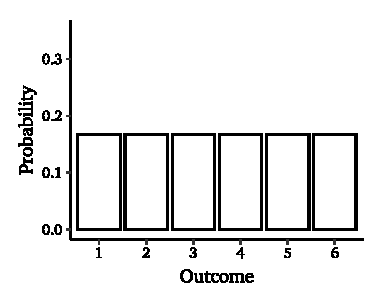
\includegraphics{./../../output/die_roll_pdf.pdf}} & 
\subfloat[Cumulative Distribution Function]{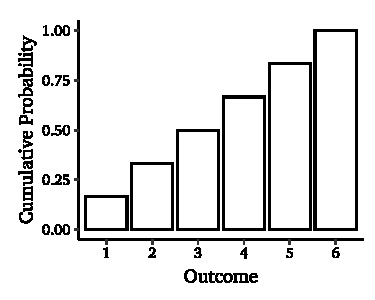
\includegraphics{./../../output/die_roll_cdf.pdf}} 
\end{tabular}
\end{figure}

\textit{Bernoulli Random Variable} is a special type of discrete random variable that only takes two values 1 and 0. It is also called a \textit{binary} variable. 

$$ X = \begin{cases} 
 	1 \quad \text{with probability $p$} \\
 	0 \quad \text{with probability $1-p$} 
 \end{cases}
$$


%%%%% Continuous Random Variables
\subsection{Continuous Random Variables}

Because of continuum of possible values, it is not feasible to list the probability of each possible value of a continuous random variable. So we instead have the \textit{probability density function} (PDF), denoted by $f(x)$. The area under the curve $f(x)$ gives us the probability of $X$ falling in certain intervals. The \textit{probability density function} is defined as:

$$ Pr(a \leq x \leq b) =  \int_{a}^{b} f(x) \partial x $$

where $f(x)>0$ for all $x$ and $\int_{-\infty}^{\infty} f(x) \partial x =1 $. 

Note that for continuous random variables, $Pr(X=x)=0$. This is just to say that it is very very unlikely that any particular value will be realized because there are infinite possibilities. 

The integral $\int^{b}_{a}$ is the continuous analog of the sum. You don't need to know how to solve an integral, but remember it is like taking a sum over continuous values. The limits of the integral, $a$ and $b$, define the interval over which we are taking this sum.

The \textit{cumulative density function} (CDF) for a continuous random variable $X$ is given by: 

$$ F(x_0) = Pr(X \leq x_0) = \int_{-\infty}^{x_0} f(x) \partial x$$

Note that, $ Pr(a \leq x \leq b) = F(b) - F(a) $. 

\textit{Example.} Let's say the distribution for the height of individuals in the world is given by the following probability density function: 

\begin{figure}[!h]
\centering
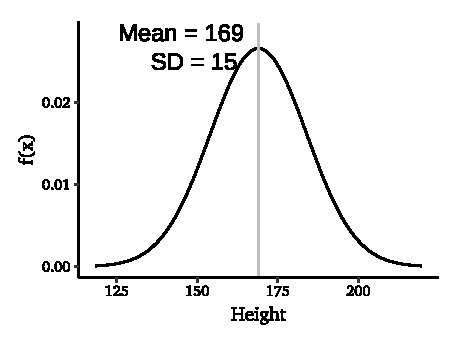
\includegraphics{./../../output/height_norm_pdf.pdf} \\
\end{figure}

We need to find the corresponding area under the curve to find the probability of height being in particular intervals. 

\begin{figure}[!h]
\begin{tabular}{cc}
\subfloat[$Pr(150<X<175)$]{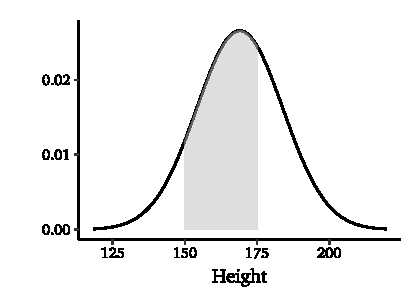
\includegraphics{./../../output/height_norm2_ho.pdf}} &
\subfloat[$Pr(X<150)$]{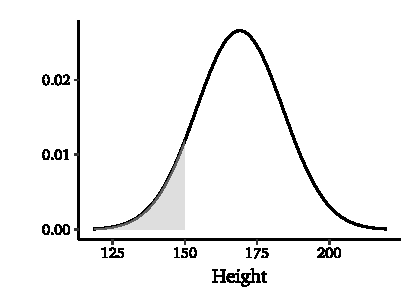
\includegraphics{./../../output/height_norm2_ho2.pdf}} 
\end{tabular}
\end{figure}

The CDF corresponding to the above PDF looks like:

\begin{figure}[!h]
\centering
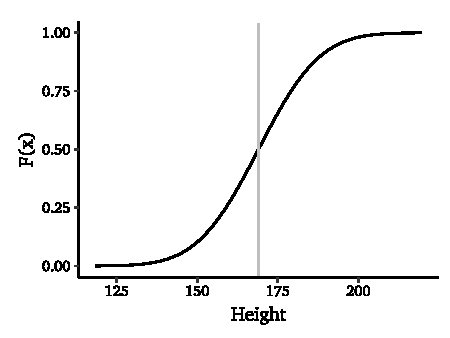
\includegraphics{./../../output/height_norm_cdf.pdf} 
\end{figure}

%%%%% Expectation and Variance
\subsection{Expectation and Variance of Random Variables}

The \textit{expectation} or \textit{expected value} or the \textit{mean} of a random variable gives us the average value of this variable over many repeated trials or occurrences. We can compute the expectation as a weighted average of possible outcomes, where the weights are probabilities.  

The expectation of a discrete random variable is given by:

$$ \mu_X = E(X) = \sum_x x f(x) $$

The expected value for a continuous random variable is given by:
$$ \mu_X = E(X) = \int_x x f(x) \partial x $$

The \textit{variance} measures the dispersion or the ``spread'' of a
probability distribution. The variance for a random variable is given by:

$$\sigma_X^2 = Var(X) = E [(X-\mu_X)^2]   $$ 

In other words, variance is the expected value of the square of deviations of $X$ from its mean. 

Using the definition of expectation for a discrete random variable, we can write:
$$\sigma_X^2 = Var(X) = E [(X-\mu_X)^2] = \sum_x (x-\mu_X)^2 f(x)  $$ 

Alternative formula for the variance:  $Var(X) = E[(X-\mu_X)^2] = E(X^2)-\mu_X^2$.

Variance is in units of the square of $X$. Therefore we use \textit{standard deviation}, which is the square-root of variance:
$$\sigma_X = \sqrt{\sigma_X^2}$$ 


\textit{Example}. We can calculate the expected value and variance for the outcome of rolling a die as follows:
\begin{center}
\begin{tabularx}{0.75\textwidth}{XXXX}
\toprule
$x$ & $f(x)$ & $xf(x)$ & $(x-\mu_X)^2 f(x)$ \\ 
\midrule
1 & 1/6 & 1/6 & (-2.5)$^2$/6 \\
2 & 1/6 & 2/6 & (-1.5)$^2$/6 \\
3 & 1/6 & 3/6 & (-0.5)$^2$/6 \\
4 & 1/6 & 4/6 & (0.5)$^2$/6 \\
5 & 1/6 & 5/6 & (1.5)$^2$/6 \\
6 & 1/6 & 6/6 & (2.5)$^2$/6 \\ \midrule
Total & - & 21/6 & 17.5/6 \\
\bottomrule
\end{tabularx}
\end{center}
$$ \mu_X = E(X) = \sum_{x} xf(x) = \frac{21}{6} = 3.5 $$ 
$$ Var(X) = \sum_x (x-\mu_X)^2 f(x) = \frac{17.5}{6} $$ 

\textit{Example}. The expected value and variance for a binary random variable that takes value 1 with probability $p$ and 0 with probability $1-p$ is given by:
$$ \mu_X = E(X) =  \sum_{x} xf(x) = 1.p + 0.(1-p) = p$$
$$ Var(X) =  \sum_{x} (x-\mu_X)^2 f(x) = (1-p)^2.p + (0-p)^2.(1-p) = p(1-p)$$
Using the alternative formula for variance:
$$ Var(X) = E(X^2)-\mu_X^2 = 1^2.p +0^2.(1-p) -\mu_X^2 = p-p^2 = p(1-p)$$

\section{Normal and Standard Normal Distribution} 

\subsection{Normal Distribution}
There are lots and lots of probability distributions that are used for modeling different variables. For example, \textit{uniform} distribution is a distribution with constant probability. There are many more, Bernoulli, binomial, gamma, beta, Poisson, and so on. 

 However, one distribution that appears over and over again is the \textit{normal distribution}. The distribution of a lot of things like height, birthweight, IQ, etc. is normal. The normal distribution is symmetric (i.e., the left and right tails are the same sizes and there’s no skew). For this reason, sometimes it is informally referred to as a bell curve. We express normal distribution with mean $\mu$ and variance $\sigma^2$ as follows:
 $$ N(\mu, \sigma^2) $$
  
Figure 2 presents normal distributions with different means and variances.  \\
 \begin{figure}[!h]\caption{Normal distributions with different means and variances}
\centering
\begin{tabular}{c}
\subfloat{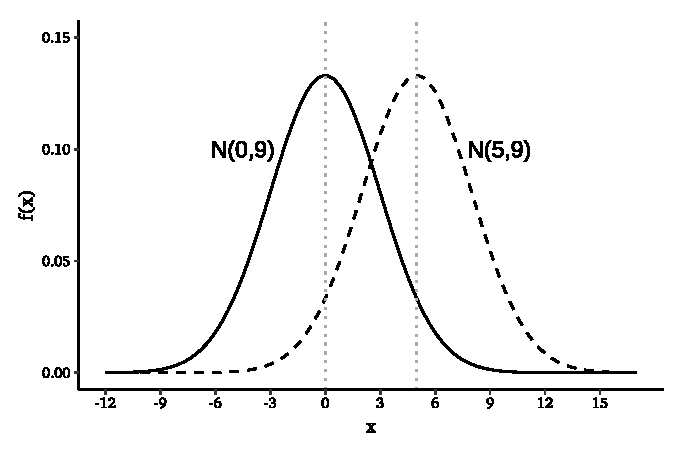
\includegraphics[scale=0.85]{./../../output/norm1}} \\
\subfloat{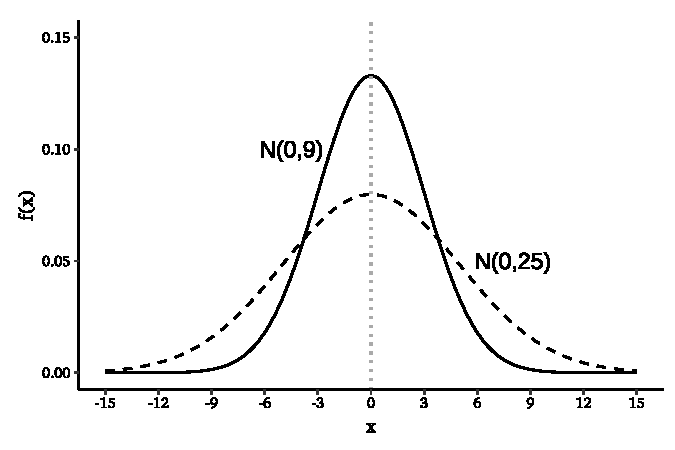
\includegraphics[scale=0.85]{./../../output/norm2.pdf}} \\
\end{tabular}
\end{figure}

The distribution of height that we saw in the above example was a normal distribution with a mean of 169 and a variance of 225. In which case, we can write $height \sim N(169, 225)$, which is short-form for saying height is normally distributed with mean 169 and variance 225. 

\subsection{Standard Normal Distribution}
The normal distribution with mean 0 and variance 1 is called the \textit{standard normal distribution} and is denoted by $N(0,1)$. Random variables that have a $N(0,1)$ distribution are often denoted by $Z$. 

In fact, we can standardize any normally distributed variable into a standard normal variable by subtracting the mean of the normal variable from each value in the distribution and then dividing by the standard deviation of the distribution. Given $X \sim N(\mu, \sigma^2)$, the standardized random variable is given by:
$$ Z = \frac{X-\mu}{\sigma} $$
Here, $Z \sim N(0,1)$. To see why this is the case, note that when we standardize $X$, we subtract the mean $\mu$ from each value of $X$. This has the effect of shifting the distribution so that its center is at 0. Next, we divide each value by the standard deviation $\sigma$. This has the effect of scaling the distribution so that its spread equals 1.

\subsection{Finding the area under the curve}

We are often interested in finding the probability that a random variable lies in a particular interval. For example, say $X \sim N(3, 16)$, and we want to calculate $Pr(X \geq 5)$. As we said before, to find this probability, we need to calculate the following area under the curve:\\

 \begin{figure}[!h]
 \centering	
\begin{tikzpicture}
\begin{axis}[
  no markers, domain=3-3*4:3+3*4, samples=100,
  axis lines*=left, xlabel=X, ylabel=$f(X)$,
  %every axis y label/.style={at=(current axis.above origin),anchor=south},
  height=4.5cm, width=8cm,
  xtick={-5, -3, -1, 1, 3, 5, 7, 9, 11}, %ytick=\empty,
  enlargelimits=false, clip=false, axis on top,
  ]
  \addplot [very thick,black] {gauss(3, 4)}; 
  \addplot [fill=gray!30, draw=none, domain=5:3+3*4] {gauss(3, 4)} \closedcycle;
%\draw[->, line width=1pt](axis cs: 185, 0.0125)--(axis cs: 205, 0.0125);
%\node at (axis cs: 0, 0.2) { 95\%};
\end{axis}
\end{tikzpicture}
 \end{figure}

However, it can be difficult and time-consuming to calculate the area by hand. Instead, we can standardize this variable and use the \textit{standard normal table} to find this area. The standard normal table provides the area under the standard normal distribution curve for different values of $Z$. 

Given $X \sim N(3, 16)$, 
$$ Z = \frac{X-3}{4} \sim N(0,1) $$

Note that, 
  $$ Pr(X \geq 5) = Pr\left(\frac{X-3}{4} \geq \frac{5-3}{4}\right) = Pr(Z \geq 0.5)  $$
 We can now refer to the standard normal table and find that $Pr(Z \geq 0.5)$ equals 0.3085. The figure below presents this probability as the area under the curve standard normal curve. \\

 \begin{figure}[!h]
 \centering	
\begin{tikzpicture}
\begin{axis}[
  no markers, domain=-3:3, samples=100,
  axis lines*=left, xlabel=Z, ylabel=$f(Z)$,
  %every axis y label/.style={at=(current axis.above origin),anchor=south},
  height=4.5cm, width=8cm,
  xtick={-1.96, 0, 0.5, 1.96}, %ytick=\empty,
  enlargelimits=false, clip=false, axis on top,
  ]
  \addplot [very thick,black] {gauss(0, 1)}; 
  \addplot [fill=gray!30, draw=none, domain=0.5:3] {gauss(0, 1)} \closedcycle;
%\draw[->, line width=1pt](axis cs: 185, 0.0125)--(axis cs: 205, 0.0125);
\end{axis}
\end{tikzpicture}
 \end{figure}


\fbox{\begin{minipage}{\textwidth}
Given $X \sim N(\mu, \sigma^2)$, general recipe to find $Pr(x_0<X<x_1)$:
\begin{itemize}
  \item Find $z_0 = (x_0-\mu)/\sigma$ and $z_1 = (x_1-\mu)/\sigma$
  \item Use standard normal table to find $Pr(z_0<Z<z_1)$ 
\end{itemize}

\end{minipage}} \\ 

\textit{Example.} Given $X \sim N(3, 16)$, we want to find $Pr(2<X<5)$. Here $x_0 = 2, x_1=5$, we can find that  $z_0 = (2-3)/4=-0.25$ and $z_1=(5-3)/4=0.5$. Now we just need to look at the standard normal table and find $Pr(-0.25<Z<0.5)$.

Alternatively, sometimes we wish to identify the value of $x$ for which the probability $Pr(X < x)$ or $Pr(X > x)$ equals a specific value $p$. This can be achieved in a similar manner by using the standard normal table. In particular, we need to find the corresponding value $z$ that satisfies $Pr(Z < z)$ or $Pr(Z > z)$, and then transform it back to obtain $x$. 

\fbox{\begin{minipage}{\textwidth}
Given $X \sim N(\mu, \sigma^2)$ and $Pr(X<x)=p$, to find $x$ : 
\begin{itemize}
  \item Use standard normal table to find $z$ where $Pr(Z<z)=p$ 
  \item Find $x = \mu + z \cdot \sigma $  
\end{itemize}
This follows analogously for when we are given $Pr(X>x)=p$.
\end{minipage}} \\ 


\section{Multiple Random Variables}

\subsection{Joint and Marginal Distribution}

The \textit{joint probability distribution} of two discrete random variables $X$ and $Y$, is the probability that the random variables simultaneously take on certain values.
$$ f(x,y) = Pr(X=x, Y=y)  $$
\vspace{0.25em}

\textit{Example}. The table below gives us the probability of possible commute times and rain on a given day. \\~\\
\begin{tabularx}{0.95\textwidth}{cccc}
\toprule
	& Rain $(X=1)$ & No Rain $(X=0)$ & Total \\
	\midrule
60-min commute ($Y=60$) & 0.3  & 0.2 & 0.5 \\ 
30-min commute ($Y=30$) & 0.1 & 0.4 & 0.5 \\
\midrule
 Total & 0.4 & 0.6 & 1 \\
 \bottomrule \\
\end{tabularx}

The \textit{marginal probability distribution} of a random variable $Y$ is just another name for its probability distribution. In particular, 
$$ f(y) = Pr(Y=y) = \sum_{x} Pr(X=x, Y=y) $$

For example, the probability of having a 60-minute commute is given by the sum of probability of having a 60-minute commute and no rain and the probability of having a 60-minute commute and rain. 
$$ Pr(Y=60) = Pr(X=1, Y=60) + Pr(X=0, Y=60) = 0.3 + 0.2 = 0.5 $$


\subsection{Conditional Probability and Bayes Rule}
The distribution of a random variable $Y$ conditional on another random variable $X$ taking on a specific value is called the \textit{conditional
distribution} of $Y$ given $X$.
$$ f(y|x) = Pr(Y=y| X=x) = \frac{Pr(X=x, Y=y)}{Pr(X=x)} = \frac{f(x,y)}{f(x)}  $$

For example, the probability of having a 60-minute commute conditional on rain is given by:
$$ Pr(Y=60| X=1) = \frac{Pr(X=1, Y=60)}{Pr(X=1)}  = \frac{0.3}{0.4} = \frac{3}{4} $$

While the probability of having a 60-minute commute conditional on no rain is given by:
$$ Pr(Y=60| X=0) = \frac{Pr(X=0, Y=60)}{Pr(X=0)}  = \frac{0.2}{0.6} =\frac{1}{3} $$

Remember, the unconditional probability of having a 60-minute commute was given by 0.5.

The \textit{conditional expectation} of $Y$ given $X$ is the mean of the conditional distribution of $Y$ given $X$. \\
$$ E(Y|X=x) = \sum_{y} y Pr(Y=y | X=x) $$

For the example above, 
$$ E(Y|X=1) = 60.Pr(Y=60 | X=1) + 30.Pr(Y=30 | X=1) = 60 \cdot \frac{3}{4} + 30 \cdot \frac{1}{4}  = 52.5 $$
Similarly,
$$ E(Y|X=0) = 60.Pr(Y=60 | X=0) + 30.Pr(Y=30 | X=0) = 60 \cdot \frac{1}{3} + 30 \cdot \frac{2}{3}  = 40 $$
So by comparing $E(Y|X=1)$ and $E(Y|X=0)$, we can find out how rain affects the average commute time. 

\textit{Bayes' rule} says that the conditional probability of $Y$ given $X$ is the conditional probability of $X$ given $Y$ times the relative marginal probabilities of $Y$ and $X$:
$$ Pr(Y=y| X=x) = \frac{Pr(X=x| Y=y)Pr(Y=y)}{Pr(X=x)}   $$

This is a very useful law because it says that we can deduce conditional probabilities from the reverse conditional probability with the help of marginal probabilities. 

\subsection{Law of Iterated Expectations}
The mean of $Y$ is the weighted average of the conditional expectation of $Y$ given $X$, weighted by the probability distribution of $X$.
$$ E(Y) = \sum_x E(Y|X=x) Pr(X=x) $$
More compactly,
$$ E(Y) = E(E(Y|X)) $$
E.g. the mean height of adults is the weighted average of the mean height
of men and women, weighted by their proportions.  

\subsection{Independence and Uncorrelatedness}

Two random variables $X$ and $Y$ are independently distributed, or \textit{independent}, if knowing the value of one of the variables provides no information about the other. That is,
$$ Pr(Y=y | X=x) = Pr(Y=y)  $$
Then by Bayes' rule:
$$ Pr(X=x, Y=y) = Pr(X=x) Pr(Y=y)  $$
\textit{Example}: Two consecutive coin tosses. \\~\\
Note: We can equivalently say that $X$ and $Y$ are independent if $E(Y|X) = E(Y)$.

\textit{Covariance} is a measure of the extent to which two random variables move
together. Let $X$ and $Y$ be a pair of random variables, then the \textit{covariance} of $X$ and $Y$ is given by:
$$ \sigma_{XY} = Cov(X,Y) = E[(X-\mu_X)(Y-\mu_Y)] = E(XY)-\mu_X \mu_Y $$ 

The \textit{correlation} between $X$ and $Y$ is given by:
$$ \rho_{XY} = corr(X,Y) = \frac{Cov(X,Y)}{\sigma_X \sigma_Y} \quad \text{ where } -1 \leq \rho \leq 1$$
$X$ and $Y$ are uncorrelated if $\rho_{XY}=\sigma_{XY}=0$ i.e. $E(XY)=E(X)E(Y)$. \\~\\

\fbox{\begin{minipage}{\textwidth}
If $X$ and $Y$ are independent, then they are also uncorrelated. 
$$ E(Y|X) = E(Y) \rightarrow \rho_{XY} = 0 $$
However, it is not necessarily true that if $X$ and $Y$ are uncorrelated, then they are also independent. 
\end{minipage}} 

%%%%%%%%%%% Linear Functions of Random Variables
\section{Linear Functions of Random Variables}

% Single Random Variable
\subsection{Linear Functions of a Single Random Variable}

If $X$ is a random variable and $Y=a+bX$, then $Y$ is also a random variable with 
$$ E(Y) = a + b E(X) \quad \quad Var(Y) = b^2 Var(X) $$ \\
In addition, a linear transformation of a random variable does not change the shape of the distribution. So if $X$ is normal, $Y$ will also be normal. \\

\textit{Example.} Let us calculate the expectation and variance for the $Z$ score:
$$ Z = \frac{X-\mu_X}{\sigma_X} $$
Note that we can write, $$ Z = -\frac{\mu_X}{\sigma_X} + \frac{1}{\sigma_X} \cdot X$$
So $a= -\frac{\mu_X}{\sigma_X}$ and $b = \frac{1}{\sigma_X}$, then by the above formulas:
$$ E(Z) = a + b E(X) =  -\frac{\mu_X}{\sigma_X} + \frac{1}{\sigma_X} \mu_X = 0 $$
$$ Var(Z) = b^2 Var(X)=   \frac{1}{\sigma_X^2} \cdot \sigma_X^2 = 1 $$
So if $X \sim N(\mu_X, \sigma^2_X)$, then $Z \sim N(0,1) $.

% Two Random Variable
\subsection{Linear Combination of Two Random Variables}
$X$ and $Y$ is a pair of random variables, define $$W= aX + bY$$
Then the expectation of $W$ is given by:
$$ E(W) = a E(X) + b E(Y) $$
And the variance of $W$ is given by:
$$ Var(W) = a^2 Var(X) + b^2 Var(Y) + 2ab Cov(X,Y) $$
If $X$ and $Y$ are independent then $Cov(X,Y)=0$, so in that case $ Var(W) = a^2 Var(X) + b^2 Var(Y) $.
% Multiple Random Variable

\subsection{Linear Combination of Several Random Variables}
 For random variables, $X_1,X_2,...,X_n$:
 $$ E(X_1 + X_2 + ... + X_n) = E(X_1) + E(X_2) + ...+ E(X_n) $$
$$ Var(X_1 + X_2 + ... + X_n) = \sum_{i=1}^n Var(X_i) + 2 \sum_{i=1}^{n-1} \sum_{j=i+1}^K Cov(X_i,X_j) $$

If $X_1,X_2,...,X_n$ are independent random variables, then $ Var\left(\sum_i X_i\right) = \sum_i Var (X_i)  $. \\

Note that a linear combination of several normally distributed random variables will also be normal.


\end{document}